\subsection{WYSIWYG}\label{wysiwyg}
�WYSIWYG� staat voor �What You See Is What You Get�. Deze functionaliteit maakt tekst opmaken en verwerken erg gemakkelijk.

\subsubsection{Koptitels}
\begin{enumerate}
\item Ga met de tekstcursor in de regel staan die een \emph{Kop 2} of \emph{Kop 3} (subkop) moet worden.
\item Klik op het Opmaak openklapmenu en kies \emph{Kop 2} of \emph{Kop 3}.
\end{enumerate}
Het is niet toegestaan om een heading 1 te gebruiken. Volgens de \emph{webrichtlijnen} is een \emph{Kop 1} altijd de paginatitel en komt deze maar 1 keer voor op een pagina. Het gebruik van koppen in teksten dient echter wel op een juiste manier te gebeuren. Gebruik niet de Vet (Bold) knop maar de Opmaak knop. Voor de hoofdkoppen in de tekst gebruikt u \emph{Kop 2}. Indien hieronder nog subkoppen gemaakt moeten worden gebruikt u \emph{Kop 3}.

\begin{center}
	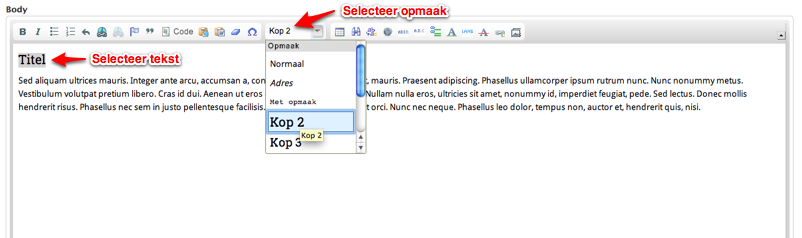
\includegraphics[width=\textwidth]{img/koptitels.png}
\end{center}

\subsubsection{Bold}
Om een bepaald woord nadruk te geven kan men de Vet (B) knop gebruiken. Gebruik deze knop niet om Headers cq koptitels te maken.
\begin{enumerate}
\item Selecteer het woord met de muis wat u vet wilt maken.
\item Klik op de B-knop.
\item Wilt u het woord niet meer vet hebben, klik dan nog een keer op de B-knop.
\end{enumerate}

\begin{center}
	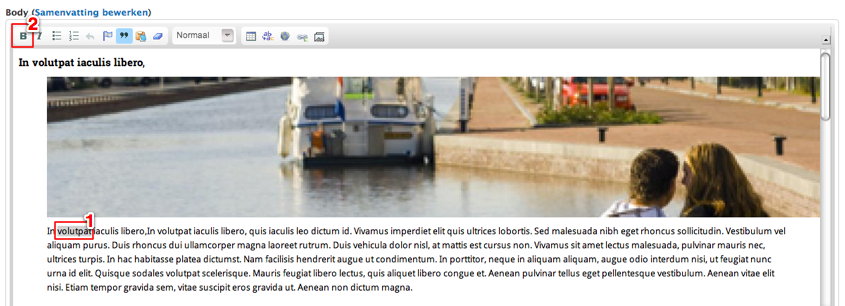
\includegraphics[width=\textwidth]{img/bold.png}
\end{center}

\subsubsection{Cursief}
Om een bepaald woord nadruk te geven kan men de \emph{Cursief} knop gebruiken, oftewel de I-knop.
\begin{enumerate}
\item Selecteer het woord met de muis wat u schuin wilt maken.
\item Klik op de I-knop.	
\item Wilt u het woord niet meer schuingedrukt hebben, klik dan nogmaals op de I-knop.
\end{enumerate}

\begin{center}
	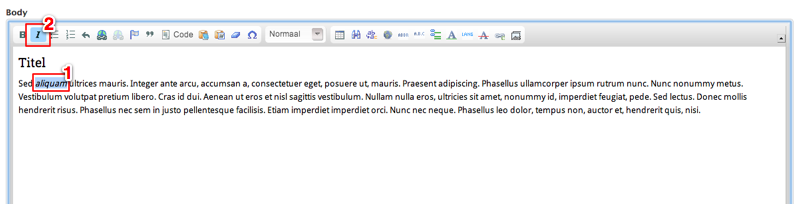
\includegraphics[width=\textwidth]{img/schuin.png}
\end{center}

\subsubsection{Opsomming}
Om een opsomming te maken kan men de Opsomming knop gebruiken.
\begin{enumerate}
\item Klik op de opsomming knop, en voer uw tekst direct in.
\item Om een nieuwe opsommingspunt te gebruiken drukt u op de Enter toets, druk 2 maal op de Enter toets om uit de opsomming te gaan.
\end{enumerate}

\begin{center}
	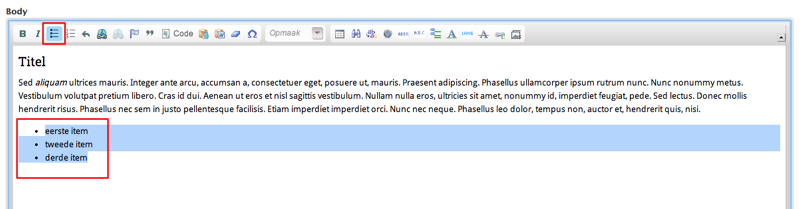
\includegraphics[width=\textwidth]{img/opsomming.png}
\end{center}

\subsubsection{Genummerde lijst}
Om een genummerde lijst te maken kan men de Genummerde lijst knop gebruiken.
\begin{enumerate}
\item Klik op de genummerde lijst knop, en voer uw tekst direct in.
\item Om een nieuw getal te gebruiken drukt u op de Enter toets, druk 2 maal op de Enter toets om uit de genummerde lijst te gaan te gaan.
\end{enumerate}

\begin{center}
	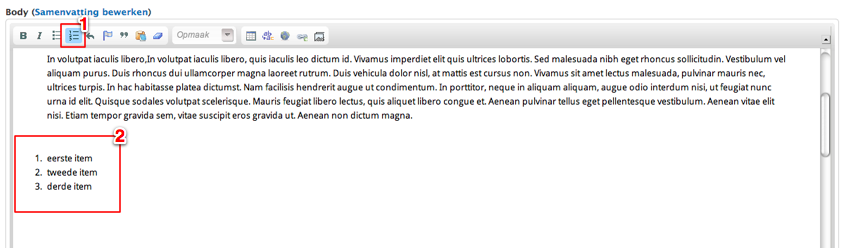
\includegraphics[width=\textwidth]{img/genummerde_lijst.png}
\end{center}

\subsubsection{Iframes}
Om een andere website te tonen op \drupalpath maken we gebruik van een iframe. Via de \emph{wereldbolknop} in 
de WYSIWYG-editor kun je een (externe)pagina tonen op een pagina van \drupalpath. Er zijn drie velden verplicht:
\begin{enumerate}
\item URL
\item Breedte
\item Hoogte
\end{enumerate}

\begin{center}
	
\includegraphics[width=\textwidth]{img/iframe1.png}
\end{center}

\subsubsection{Afkortingen}
Via de \emph{afkorting knop} kan een afkorting aangemaakt worden. Als je met de muis over de afkorting gaat zal de betekenis getoond worden.
\begin{center}
	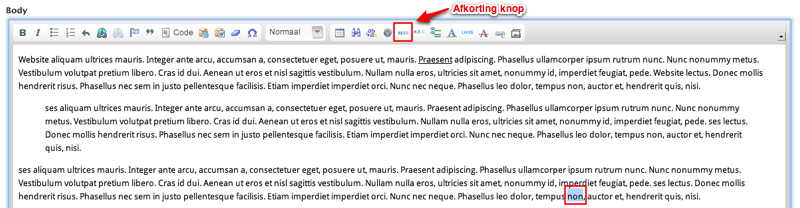
\includegraphics[width=\textwidth]{img/afkorting1.png}
	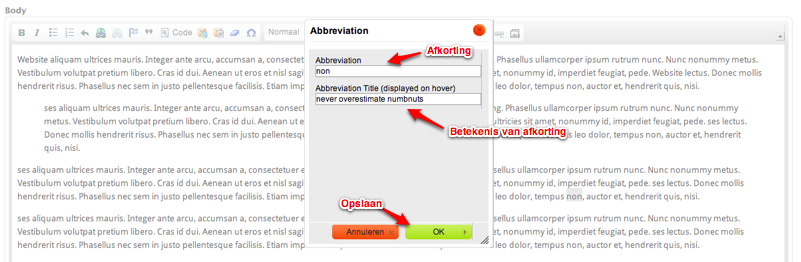
\includegraphics[width=\textwidth]{img/afkorting2.png}
\end{center}

De onderstaande afbeelding toont het resultaat.
\begin{center}
	
\includegraphics[width=\textwidth]{img/afkorting3.png}
\end{center}

\subsubsection{Acroniem}
\emph{Een acroniem of letterwoord is een afkorting die wordt uitgesproken als een woord.} Bijvoorbeeld \emph{GPS} spreekt men vrijwel altijd uit als \emph{GPS}, maar betekent in werkelijkheid \emph{Global Positioning System}.
Via de \emph{acroniem knop} kan een acroniem aangemaakt worden. Als je met de muis over een acroniem gaat zal de betekenis getoond worden.
\begin{center}
	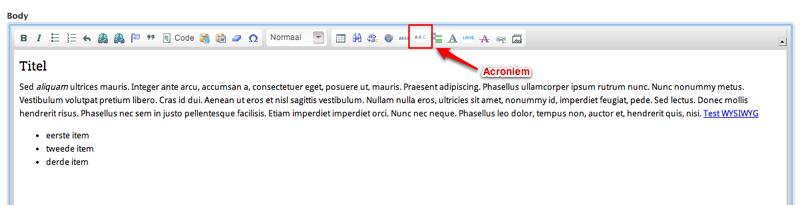
\includegraphics[width=\textwidth]{img/acroniem.png}
	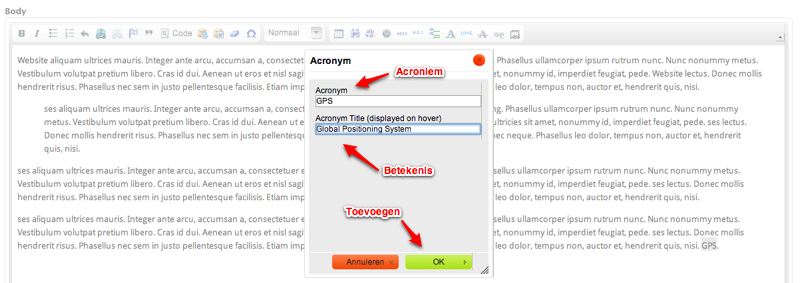
\includegraphics[width=\textwidth]{img/acroniem2.png}
	
\includegraphics[width=\textwidth]{img/acroniem3.png}
\end{center}

\subsubsection{Tabellen}
Via de \emph{tabel knop} kan een tabel worden ingevoegd. 
\begin{center}
	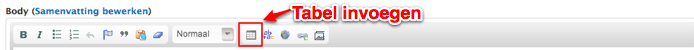
\includegraphics[width=\textwidth]{img/tabellen1.png}
\end{center}
Nadat je op de \emph{tabel knop} hebt geklikt verschijnt er een dialoog met verschillende opties. Als je klaar bent met het invullen van de tabel opties, klik dan op de knop \emph{OK} om de tabel in te voegen. De onderstaande afbeelding licht de opties in het kort toe.
\begin{center}
	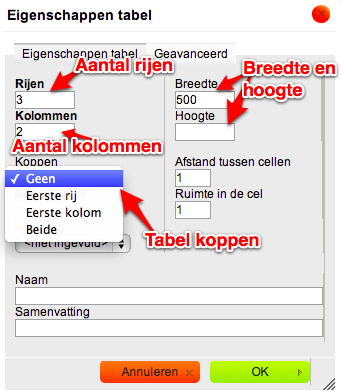
\includegraphics[width=\textwidth]{img/tabellen2.png}
\end{center}

\subsubsection{Citaatblok}
Met de \emph{Citaatblok knop} kun je een alinea extra laten opvallen. 
Klik op de gewenste alinea en klik vervolgens op de \emph{Citaatblok knop}.
\begin{center}
	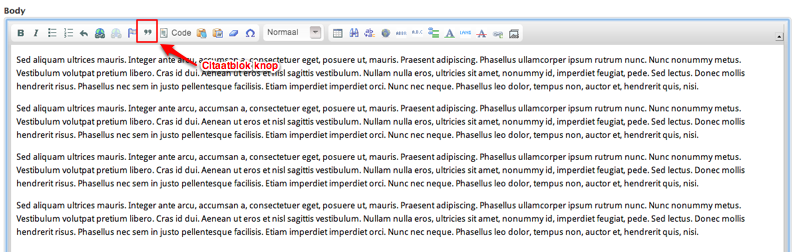
\includegraphics[width=\textwidth]{img/citaatblok.png}
\end{center}

De onderstaande afbeelding toont een voorbeeld waarbij de tweede alinea opvallender is gemaakt met de \emph{citaatblok knop}.

\begin{center}
	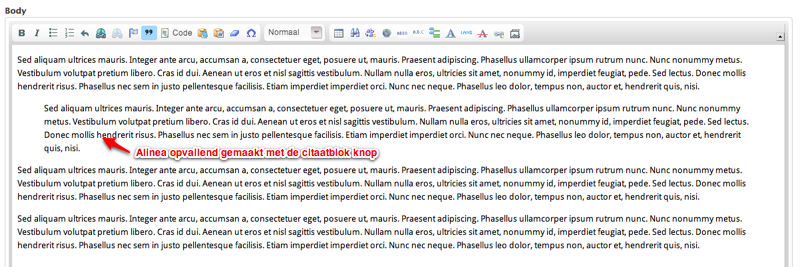
\includegraphics[width=\textwidth]{img/citaatblok2.png}
\end{center}

\subsubsection{Plakken uit word}
\begin{enumerate}
\item Kopieer de tekst van je \emph{Word document}.
\item Klik op de \emph{Plakken uit word knop}.
\item Plak de gekopieerde tekst in het tekstveld.
\item Klik op de knop \emph{OK} om de tekst in te voegen.
\end{enumerate}
\begin{center}
	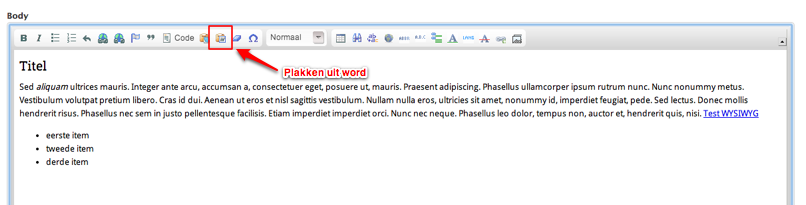
\includegraphics[width=\textwidth]{img/plakken_uit_word.png}
\end{center}

\subsubsection{Invoegen van woord}
Gebruik de \emph{invoegen van woord knop} om een woord te onderstrepen.
\begin{center}
	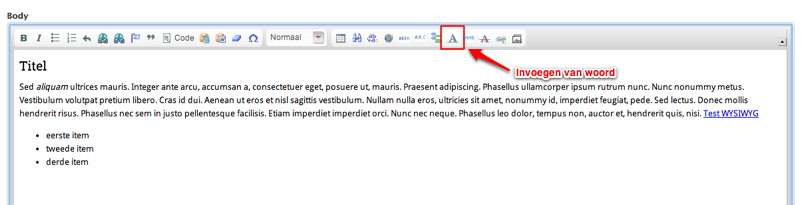
\includegraphics[width=\textwidth]{img/invoegen_van_woord.png}
\end{center}

\subsubsection{Verwijderen van woord}
Gebruik de \emph{verwijderen van woord knop} om een woord te doorstrepen.
\begin{center}
	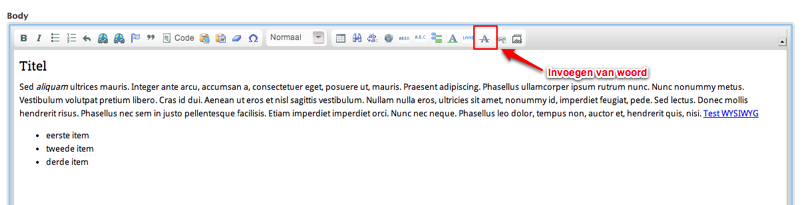
\includegraphics[width=\textwidth]{img/verwijderen_van_woord.png}
\end{center}

\subsubsection{Zoek en vervang}
Met de \emph{zoek en vervang} knop kun je in een paar handelingen specifieke woorden of zinnen vervangen.
De onderstaande afbeelding laat zien hoe dit moet.
\begin{center}
	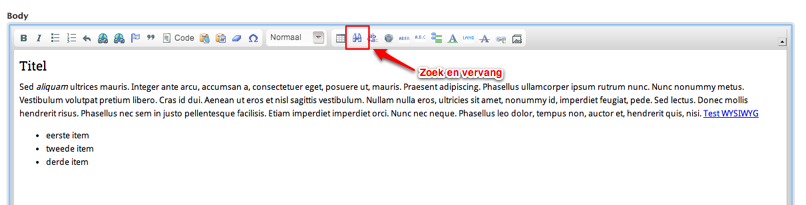
\includegraphics[width=\textwidth]{img/zoek_en_vervang.png}
	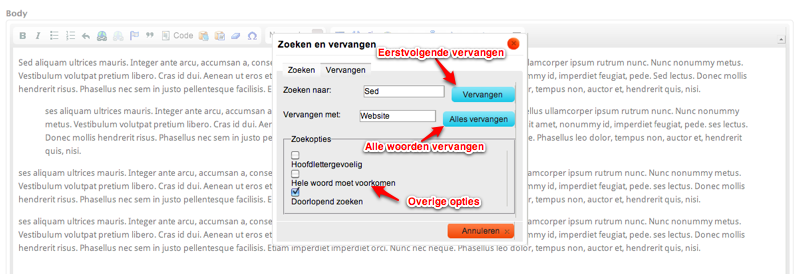
\includegraphics[width=\textwidth]{img/zoek_en_vervang2.png}
\end{center}

\subsubsection{Taal veranderen per woord}

\begin{center}
	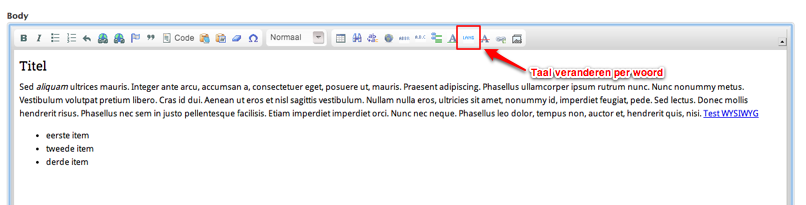
\includegraphics[width=\textwidth]{img/taal_veranderen_per_woord.png}
\end{center}

\subsubsection{Ongedaan maken}
Met de \emph{ongedaan maken knop} kun je alle wijzigingen, \emph{die nog niet zijn opgeslagen}, stap voor stap (wijziging voor wijziging) ongedaan maken. 
\begin{center}
	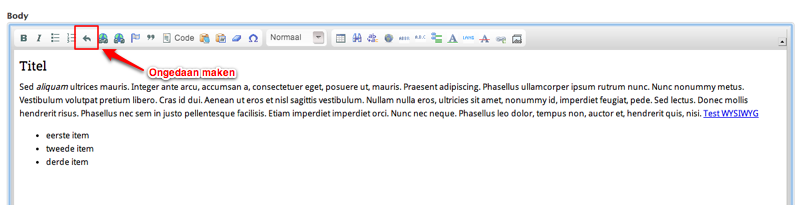
\includegraphics[width=\textwidth]{img/ongedaan_maken.png}
\end{center}

\subsubsection{Speciaal teken invoegen}
Met de \emph{Speciaal teken knop} kun je speciale tekens toevoegen aan de tekst. Klik op de \emph{Speciaal teken knop} en selecteer het gewenste teken, het teken zal gelijk worden ingevoegd.
\begin{center}
	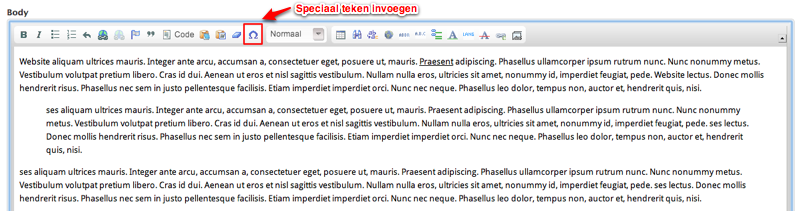
\includegraphics[width=\textwidth]{img/speciaal_teken_invoegen.png}
\end{center}

\subsubsection{Definitie lijst}
Met de \emph{definitie lijst knop} kun je lijsten maken met definities. Definitie lijsten kun je bijvoorbeeld onderaan de tekst toevoegen om bronnen e.d. te vermelden.
De onderstaande afbeeldingen geven weer hoe dit in zijn werking gaat.
\begin{center}
	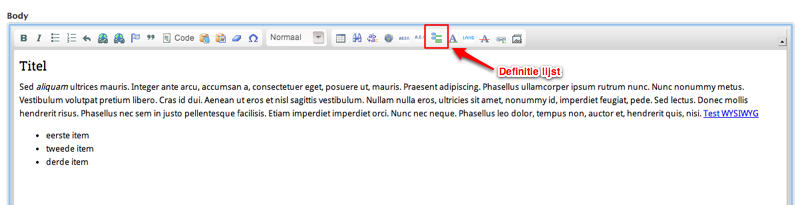
\includegraphics[width=\textwidth]{img/definitie_lijst.png}
	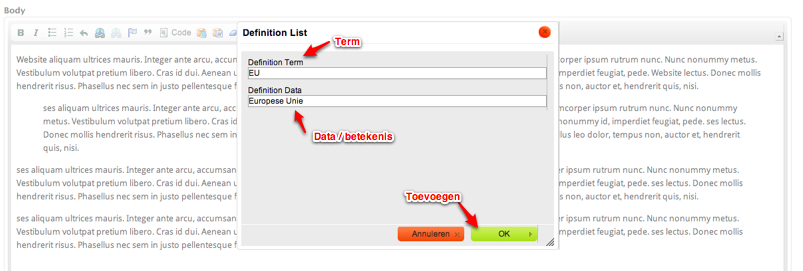
\includegraphics[width=\textwidth]{img/definitie_lijst2.png}
	
\includegraphics[width=\textwidth]{img/definitie_lijst3.png}
\end{center}


\subsubsection{(Externe)Links}
De Linkit module zorgt voor een makkelijke methode om links in content te plaatsen.  

Er zijn twee methoden beschikbaar om links in content te plaatsen. \emph{Methode 1} maakt het mogelijk hele woorden of zinnen naar een (externe)pagina te linken. \emph{Methode 2} maakt het mogelijk een \emph{harde link} te plaatsen; de link is met deze methode dan gelijk aan het opgegeven pad(URL), de bijbehorende afbeelding zal dit visueel uitleggen. Indien je met \emph{methode 2} een link maakt naar een \emph{interne pagina} dan zal de titel van pagina gebruikt worden voor de klikbare link. 

\textbf{Methode 1:} 

\begin{enumerate}
\item Selecteer het woord of de zin die je wilt \emph{linken}.
\item Druk op het \emph{Linkit} knopje.
\item Zoek in het eerste veld op interne content, indien gevonden, klik op de gevonden titel.
\item Indien je zelf een URL wil invullen, bijvoorbeeld een externe, vul deze dan in bij het veld \emph{Link-url}.
\item Klik op de knop \emph{Link invoegen} om te link toe te voegen aan de content.
\end{enumerate}

\begin{center}
	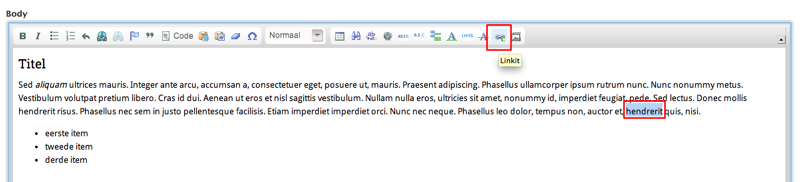
\includegraphics[width=\textwidth]{img/linkit1.png}
	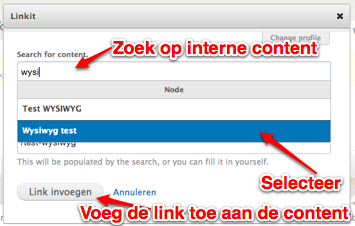
\includegraphics[width=\textwidth]{img/linkit2.png}
	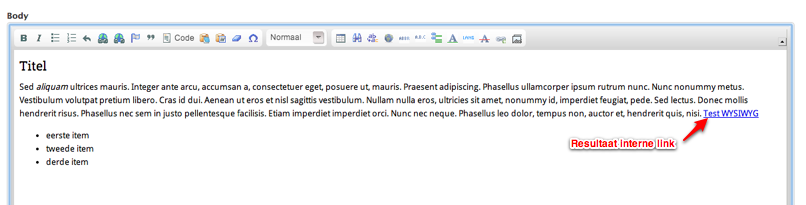
\includegraphics[width=\textwidth]{img/linkit4.png}
\end{center}

\textbf{Methode 2:} 

\begin{enumerate}
\item Druk op het \emph{Linkit} knopje.
\item Zoek in het eerste veld op interne content, indien gevonden, klik op de gevonden titel.
\item Indien je zelf een URL wil invullen, bijvoorbeeld een externe, vul deze dan in bij het veld \emph{Link-url}.
\item Klik op de knop \emph{Link invoegen} om te link toe te voegen aan de content.
\end{enumerate}

\begin{center}
	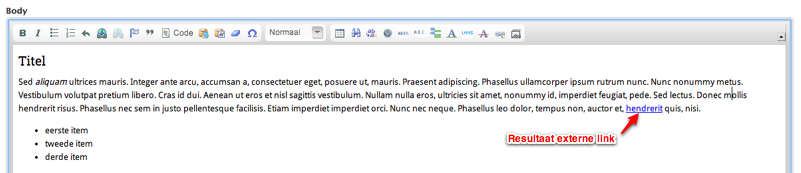
\includegraphics[width=\textwidth]{img/linkit3.png}
\end{center}

\subsubsection{(Anker) Links}\label{ankers}
Ankers kunnen gebruikt worden om naar bepaalde delen in de content te springen om zo bijvoorbeeld inhoudsopgavelijsten te maken.

Voordat er gerefereerd kan worden naar een anker moet deze eerst aangemaakt worden op de pagina. 

\begin{enumerate}
\item Plaats de cursor ergens in de content of selecteer een stuk tekst en klik op de knop \emph{Anker aanmaken}.
\item Geef een naam op, deze mag niet beginnen met een cijfer.
\item Selecteer een stuk tekst en klik op de knop \emph{Link bewerken/wijzigen}.
\item Kies vervolgens bij \emph{Linktype} voor Interne link in pagina.
\item Kies vervolgens bij \emph{Op naam interne link} een van de aanwezige ankers.
\end{enumerate}

\begin{center}
	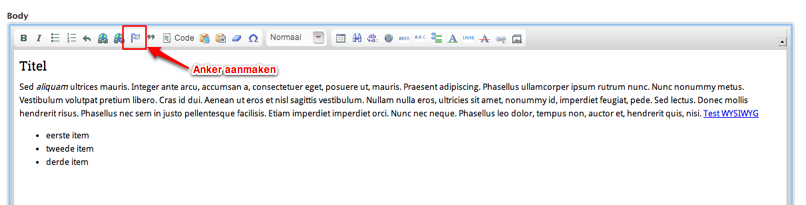
\includegraphics[width=\textwidth]{img/anker1.png}
	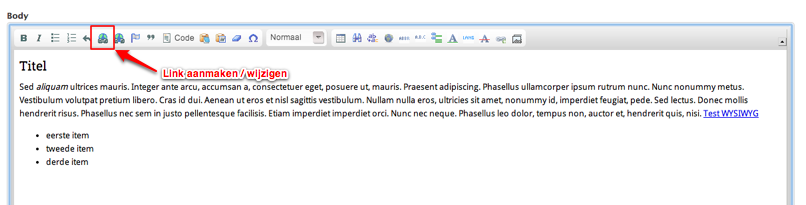
\includegraphics[width=\textwidth]{img/anker2.png}
\end{center}

\subsubsection{YouTube Embed via WYSIWYG}
\begin{enumerate}
\item Klik op de media button.
\item Vul de volledige YouTube url in.
\item Klik op de knop \emph{Indienen}.
\item Kies vervolgens bij \emph{display as} voor origineel.
\item Klik op de knop \emph{Indienen} om de Youtube video in de tekst te plaatsen.
\end{enumerate}

\begin{center}
	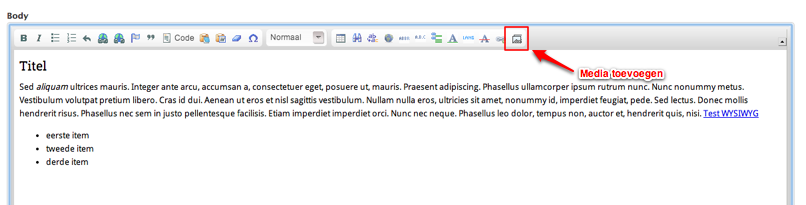
\includegraphics[width=\textwidth]{img/wysiwyg_add_media_button.png}
	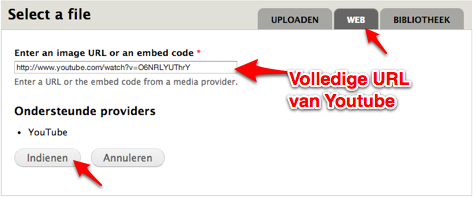
\includegraphics[width=\textwidth]{img/youtube0.png}
\end{center}

\subsubsection{YouTube Embed via Full HTML}
Let op: alleen eindredacteuren kunnen Full HTML nodes wijzigen.
\begin{enumerate}
\item Kopieer de iframe-insluitcode van Youtube.
\item Ga naar de node waarin je een Youtube video wil embedden.
\item Selecteer bij tekstopmaak \emph{Plain text}.
\item Plak de gekopieerde iframe-insluitcode op de plek waar je de Youtube video wil embedden.
\item Selecteer bij tekstopmaak \emph{Full HTML}.
\item Voer eventueel andere wijzigingen door en klik vervolgens onderaan de pagina op de knop \emph{Opslaan}.
\end{enumerate}

\begin{center}
	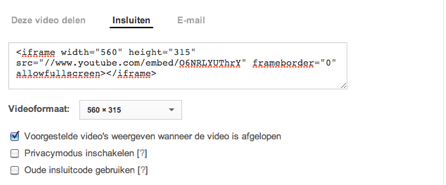
\includegraphics[width=\textwidth]{img/youtube1.png}
	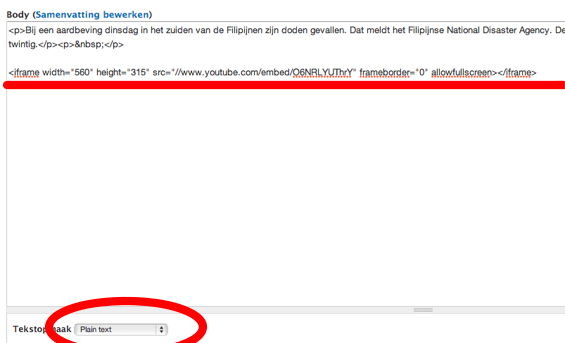
\includegraphics[width=\textwidth]{img/youtube2.png}
	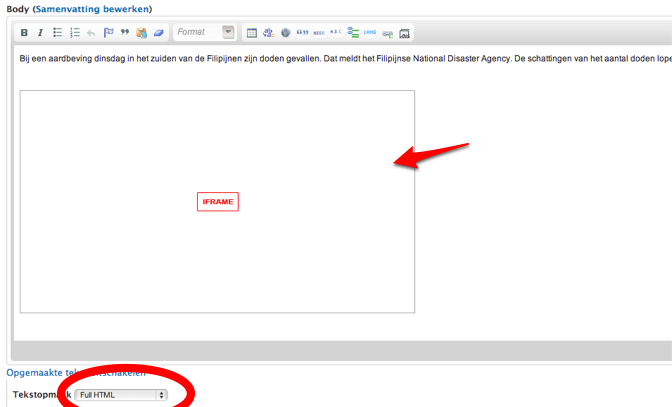
\includegraphics[width=\textwidth]{img/youtube3.png}
\end{center}

\subsubsection{Media invoegen}

Met de \emph{Media knop} kun je verschillende soorten media invoegen. Er bestaan drie methoden om Media in te voegen: \emph{uploaden vanaf de computer}, \emph{insluiten(embedden) vanaf het web} en \emph{invoegen vanuit de bibliotheek}. Je kunt bijvoorbeeld afbeeldingen, audio en tekstbestanden uploaden en Youtube video's insluiten.  De onderstaande afbeelding laat zien waar je de \emph{Media knop} kunt vinden in de \emph{WYSIWYG Editor}.

\begin{center}
	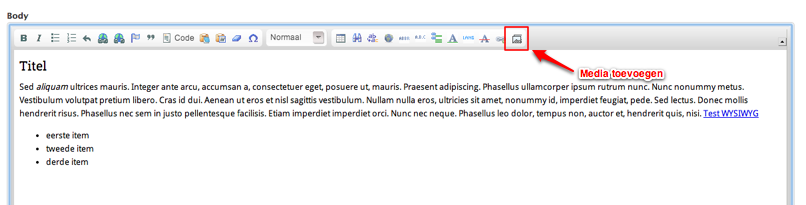
\includegraphics[width=\textwidth]{img/wysiwyg_add_media_button.png}
\end{center}

Nadat je op de knop hebt geklikt zal er een dialoog verschijnen. De onderstaande afbeelding laat het dialoog zien. 

 \begin{center}
	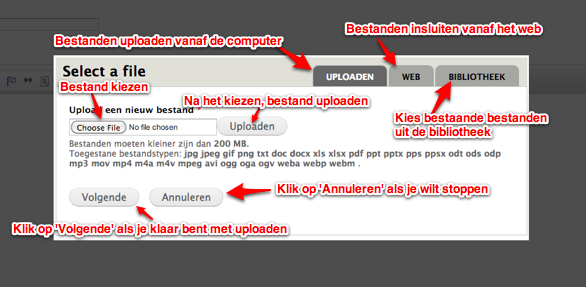
\includegraphics[width=\textwidth]{img/wysiwyg_add_media_dialog.png}
\end{center}

Per methode zal de werkwijze stap voor stap door middel van afbeeldingen beschreven worden. 

\paragraph{Media uploaden vanaf de computer}

De onderstaande afbeeldingen laten zien hoe je door middel van uploaden een afbeelding kunt toevoegen aan de tekst.

 \begin{center}
	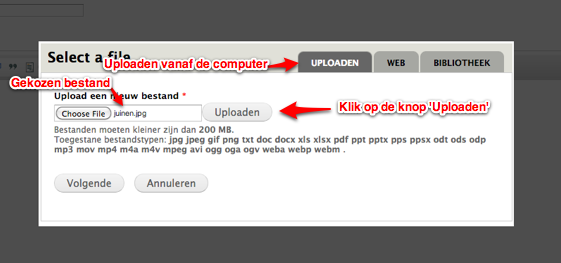
\includegraphics[width=\textwidth]{img/invoegen_upload_1.png}
	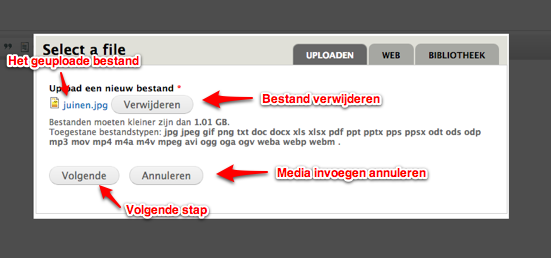
\includegraphics[width=\textwidth]{img/invoegen_upload_2.png}
	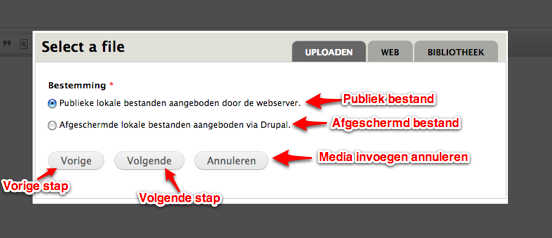
\includegraphics[width=\textwidth]{img/invoegen_upload_3.png}
	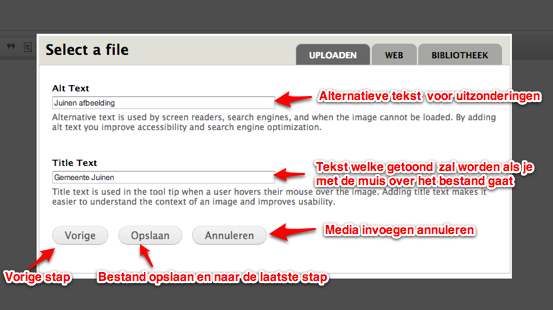
\includegraphics[width=\textwidth]{img/invoegen_upload_4.png}
	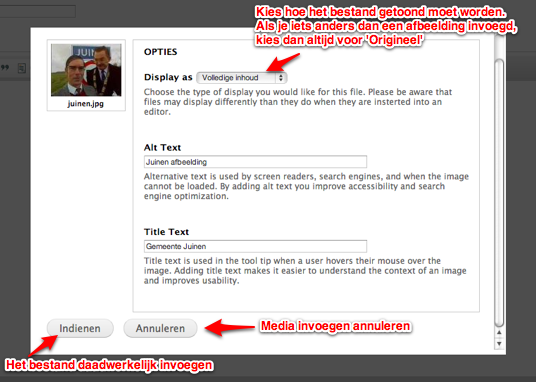
\includegraphics[width=\textwidth]{img/invoegen_upload_5.png}
	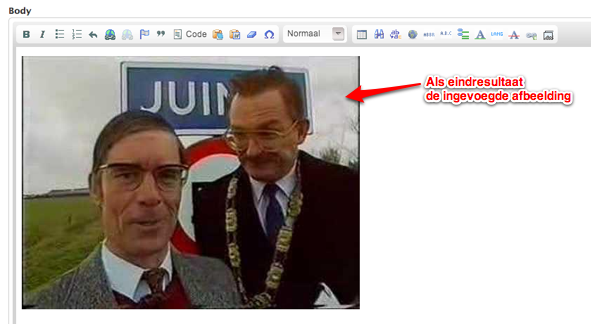
\includegraphics[width=\textwidth]{img/invoegen_upload_6.png}
\end{center}

De onderstaande afbeeldingen laten zien hoe je door middel van de methode \emph{uploaden} een \emph{Document} kunt toevoegen aan de tekst.

 \begin{center}
	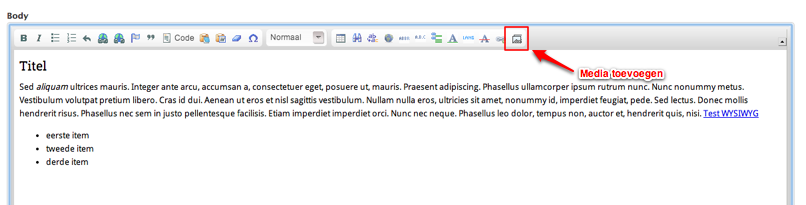
\includegraphics[width=\textwidth]{img/wysiwyg_add_media_button.png}
	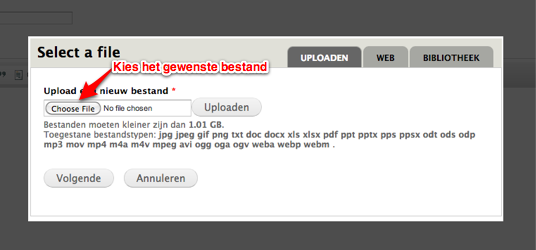
\includegraphics[width=\textwidth]{img/invoegen_upload_document_1.png}
	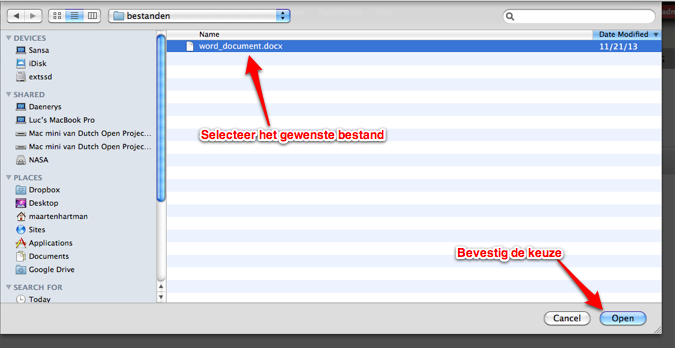
\includegraphics[width=\textwidth]{img/invoegen_upload_document_2.png}
	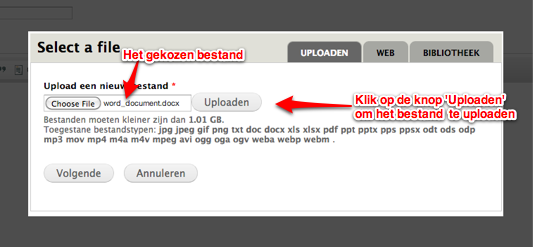
\includegraphics[width=\textwidth]{img/invoegen_upload_document_3.png}
	\includegraphics[width=\textwidth]{img/invoegen_upload_document_4.png}
	\includegraphics[width=\textwidth]{img/invoegen_upload_3.png}
	\includegraphics[width=\textwidth]{img/invoegen_upload_document_5.png}
	\includegraphics[width=\textwidth]{img/invoegen_upload_document_6.png}
\end{center}



\paragraph{Media vanaf het web}

 \begin{center}
	\includegraphics[width=\textwidth]{img/invoegen_web_1.png}
	\includegraphics[width=\textwidth]{img/invoegen_web_2.png}
\end{center}

\paragraph{Media vanuit de bibliotheek}

 \begin{center}
	\includegraphics[width=\textwidth]{img/invoegen_bibliotheek_1.png}
	\includegraphics[width=\textwidth]{img/invoegen_bibliotheek_2.png}
	\includegraphics[width=\textwidth]{img/invoegen_bibliotheek_3.png}
\end{center}
